\chapter{B\'{e}zier Intersection Problems}\label{chap:bezier-intersection}

\section{Intersecting B\'{e}zier Curves}

The problem of intersecting two B\'{e}zier curves is a core building
block for intersecting two B\'{e}zier triangles in \(\reals^2\)
Since a curve is an algebraic variety of dimension one,
the intersections will either be a curve segment common to both curves (if
they coincide) or a finite set of points (i.e. dimension zero).
Many algorithms have been described in the literature, both
geometric (\cite{Sederberg1986, Sederberg1990, Kim1998}) and
algebraic (\cite{Manocha:CSD-92-698}).

In the implementation for this work, the B\'{e}zier subdivision
algorithm is used.
In the case of a transversal intersection (i.e. one where the
tangents to each curve are not parallel and both are non-zero),
this algorithm performs very well. However, when curves are tangent,
a large number of (false) candidate intersections are detected and
convergence of Newton's method slows once in a neighborhood of an
actual intersection. Non-transversal intersections
have infinite condition number, but transversal intersections with
very high condition number can also cause convergence problems.

\begin{figure}
  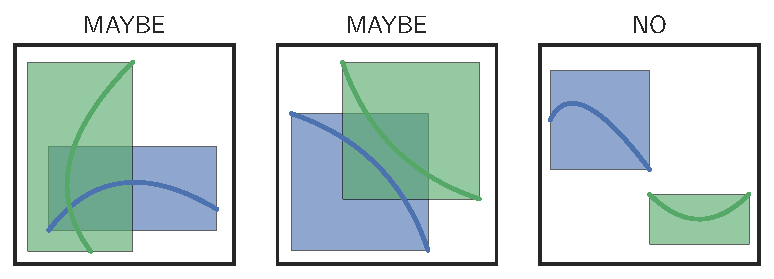
\includegraphics{../images/curved-mesh/bbox_check.pdf}
  \centering
  \captionsetup{width=.75\linewidth}
  \caption{Bounding box intersection predicate. This is a cheap way to
    conclude that two curves don't intersect, though it inherently is
    susceptible to false positives.}
  \label{fig:bounding-box-check}
\end{figure}

In the B\'{e}zier subdivision algorithm, we first check if the
bounding boxes for the curves are disjoint
(Figure~\ref{fig:bounding-box-check}).
We use the bounding boxes
rather than the convex hulls since they are easier to compute and
the intersections of boxes are easier to check.
If they are disjoint, the pair can be rejected. If not, each curve
\(\mathcal{C} = b\left(\left[0, 1\right]\right)\) is split into two halves
by splitting the unit interval: \(b\left(\left[0, \frac{1}{2}\right]\right)\)
and \(b\left(\left[\frac{1}{2}, 1\right]\right)\)
(Figure~\ref{fig:bezier-curve-subdivision}).

\begin{figure}
  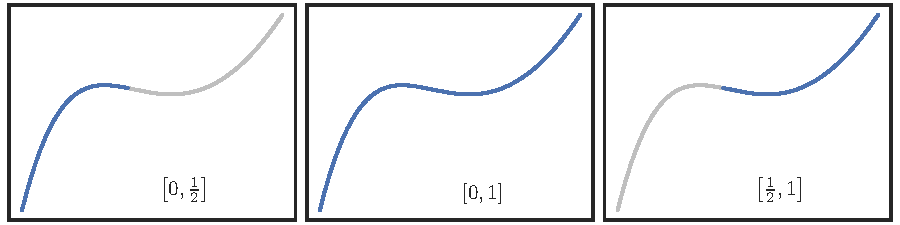
\includegraphics{../images/curved-mesh/subdivide_curve.pdf}
  \centering
  \captionsetup{width=.75\linewidth}
  \caption{B\'{e}zier curve subdivision.}
  \label{fig:bezier-curve-subdivision}
\end{figure}

\begin{figure}
  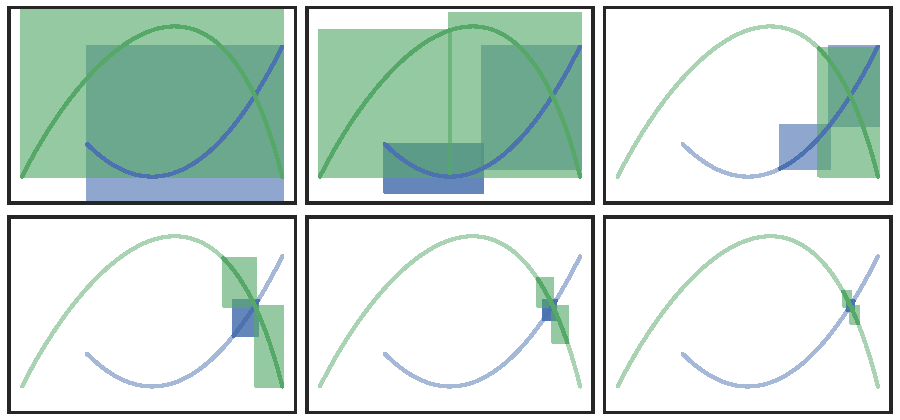
\includegraphics{../images/curved-mesh/subdivision_process.pdf}
  \centering
  \captionsetup{width=.75\linewidth}
  \caption{B\'{e}zier subdivision algorithm.}
  \label{fig:bezier-subdivision-process}
\end{figure}

As the subdivision continues,
some pairs of curve segments may be kept around that won't lead to an
intersection (Figure~\ref{fig:bezier-subdivision-process}).
Once the curve segments are close to linear within a given tolerance
(Figure~\ref{fig:bezier-subdivision-linearized}), the process
terminates.

\begin{figure}
  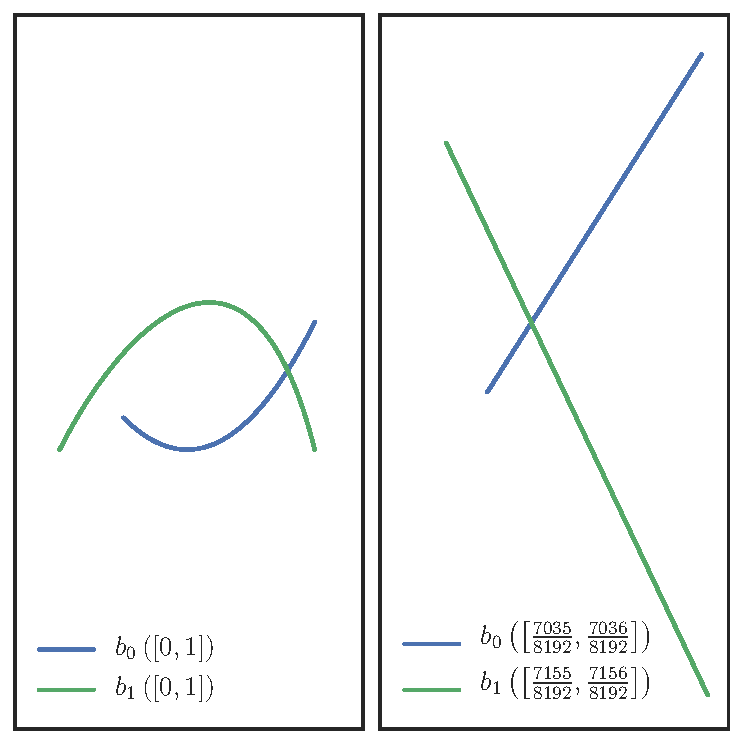
\includegraphics{../images/curved-mesh/subdivision_linearized.pdf}
  \centering
  \captionsetup{width=.75\linewidth}
  \caption{Subdividing until linear within tolerance.}
  \label{fig:bezier-subdivision-linearized}
\end{figure}

Once both curve segments are linear (to tolerance), the intersection is
approximated by intersecting the lines connecting the endpoints of each
curve segment. This approximation is used as a starting point for Newton's
method, to find a root of \(F(s, t) = b_0(s) - b_1(t)\). Since
\(b_0(s), b_1(t) \in \reals^2\) we have Jacobian \(J =
\left[ \begin{array}{c c} b_0'(s) & -b_1'(t) \end{array}\right]\).
With these, Newton's method is
\begin{equation}
\left[ \begin{array}{c c} s_{n + 1} & t_{n + 1} \end{array}\right]^T =
\left[ \begin{array}{c c} s_n & t_n \end{array}\right]^T -
J_n^{-1} F_n.
\end{equation}
This also gives an indication why convergence issues occur at non-transveral
intersections: they are exactly the intersections where the Jacobian is
singular.

\section{Intersecting B\'{e}zier Triangles}\label{sec:intersect-bez-tri}

The chief difficulty in intersecting two surfaces is intersecting their edges,
which are B\'{e}zier curves.
Though this is just a part of the overall algorithm, it proved to be the
\textbf{most difficult} to implement (\cite{Hermes2017}). So the first part
of the algorithm is to find all points
where the edges intersect (Figure~\ref{fig:edge-intersections}).

\begin{figure}
  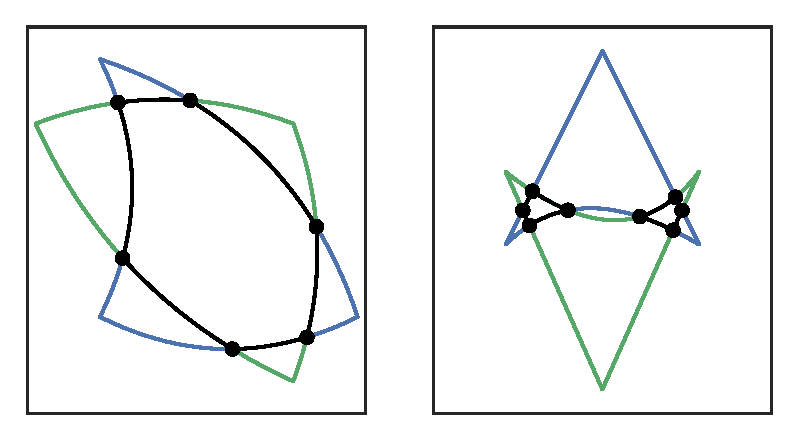
\includegraphics{../images/curved-mesh/main_figure21.pdf}
  \centering
  \captionsetup{width=.75\linewidth}
  \caption{Edge intersections during B\'{e}zier triangle intersection.}
  \label{fig:edge-intersections}
\end{figure}

To determine the curve segments that bound the curved polygon region(s)
(see Section~\ref{subsec:curved-polygons} for more about curved polygons) of
intersection, we not only need to keep track
of the coordinates of intersection, we also need to keep note of
\textbf{which} edges the intersection occurred on and the parameters along
each curve.
With this information, we can classify each point of intersection
according to which of the two curves forms the boundary of the
curved polygon (Figure~\ref{fig:intersection-classification}).
Using the right-hand rule we can compare the tangent
vectors on each curve to determine which one is on the interior.

\begin{figure}
  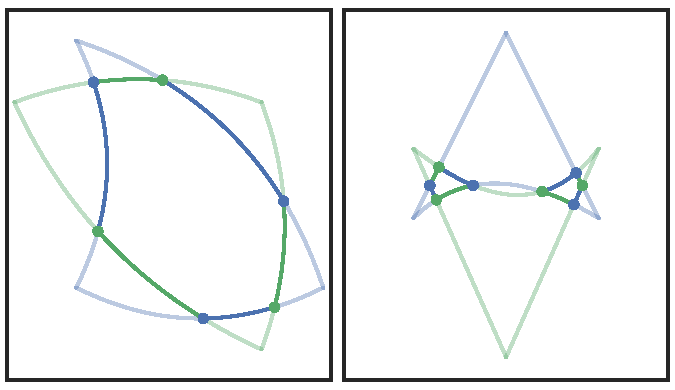
\includegraphics{../images/curved-mesh/main_figure22.pdf}
  \centering
  \captionsetup{width=.75\linewidth}
  \caption{Classified intersections during B\'{e}zier triangle intersection.}
  \label{fig:intersection-classification}
\end{figure}

This classification becomes more difficult when the curves
are tangent at an intersection, when the intersection occurs at a corner
of one of the surfaces or when two intersecting edges are coincident
on the same algebraic curve (Figure~\ref{fig:intersection-difficulties}).

\begin{figure}
  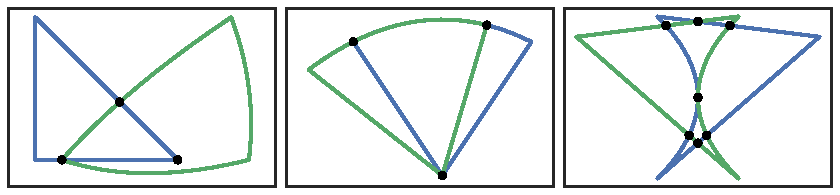
\includegraphics{../images/curved-mesh/main_figure23.pdf}
  \centering
  \captionsetup{width=.75\linewidth}
  \caption{B\'{e}zier triangle intersection difficulties.}
  \label{fig:intersection-difficulties}
\end{figure}

In the case of tangency, the intersection is non-transversal, hence has
infinite condition number. In the case of coincident curves, there are
infinitely many intersections (along the segment when the curves
coincide) so the subdivision process breaks down.

\subsection{Example}

Consider two B\'{e}zier surfaces
(Figure~\ref{fig:surface-surface-example})

\begin{equation}
b_0(s, t) =
\left[ \begin{array}{c}
    8 s \\ 8 t \end{array}\right] \qquad
b_1(s, t) =
\left[ \begin{array}{c}
    2 (6 s + t - 1) \\
    2 (8 s^2 + 8 s t - 8 s + 3 t + 2) \end{array}\right]
\end{equation}
\begin{figure}
  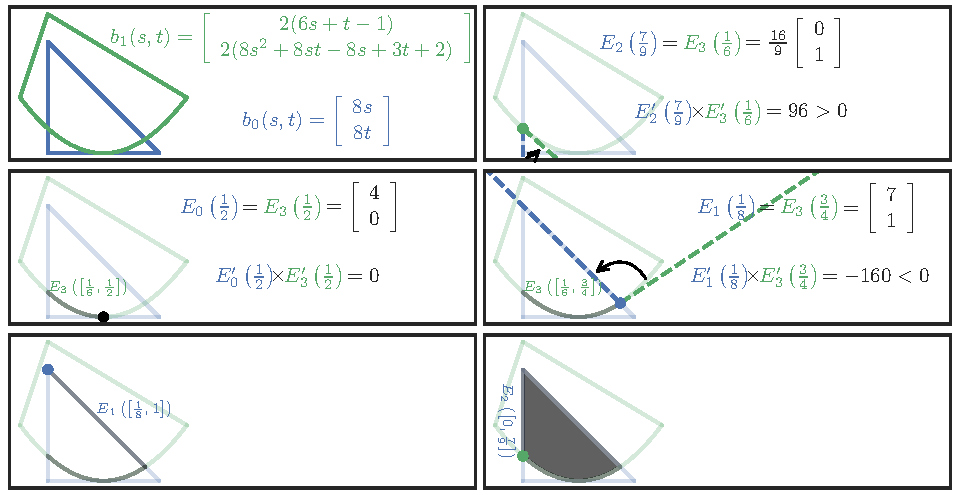
\includegraphics{../images/curved-mesh/main_figure24.pdf}
  \centering
  \captionsetup{width=.75\linewidth}
  \caption{Surface Intersection Example}
  \label{fig:surface-surface-example}
\end{figure}

In the \textbf{first step} we find all intersections of the
edge curves
\begin{multline}
E_0(r) = \left[ \begin{array}{c} 8 r \\ 0 \end{array}\right],
E_1(r) = \left[ \begin{array}{c} 8 (1 - r) \\ 8 r \end{array}\right],
E_2(r) = \left[ \begin{array}{c} 0 \\ 8 (1 - r) \end{array}\right], \\
E_3(r) = \left[ \begin{array}{c} 2 (6 r - 1) \\ 4 (2 r - 1)^2
  \end{array}\right],
E_4(r) = \left[ \begin{array}{c} 10 (1 - r) \\ 2 (3 r + 2) \end{array}\right],
E_5(r) = \left[ \begin{array}{c} - 2 r \\ 2 (5 - 3 r) \end{array}\right].
\end{multline}
We find three intersections
and we classify each of them by comparing the tangent vectors
\begin{gather}
  I_1:
  E_2\left(\frac{7}{9}\right) =
E_3\left(\frac{1}{6}\right) = \frac{16}{9}
\left[ \begin{array}{c} 0 \\ 1 \end{array}\right] \Longrightarrow
E_2'\left(\frac{7}{9}\right) \times
E_3'\left(\frac{1}{6}\right) = 96 \\
I_2:
E_0\left(\frac{1}{2}\right) =
E_3\left(\frac{1}{2}\right) =
\left[ \begin{array}{c} 4 \\ 0 \end{array}\right] \Longrightarrow
E_0'\left(\frac{1}{2}\right) \times
E_3'\left(\frac{1}{2}\right) = 0 \\
  I_3:
E_1\left(\frac{1}{8}\right) =
E_3\left(\frac{3}{4}\right) =
\left[ \begin{array}{c} 7 \\ 1 \end{array}\right] \Longrightarrow
E_1'\left(\frac{1}{8}\right) \times
E_3'\left(\frac{3}{4}\right) = -160.
\end{gather}
From here, we construct our curved polygon intersection by drawing
from our list of intersections until none remain.

\begin{itemize}
\itemsep 0em
\item First consider \(I_1\). Since
  \(E_2' \times
  E_3' > 0\)
  at this point, then we consider the curve
  \(E_3\) to be
  \textit{interior}.
\item After classification, we move along
  \(E_3\) until we
  encounter another intersection: \(I_2\)
\item \(I_2\) is a point of tangency since
  \(E_0'\left(\frac{1}{2}\right) \times
  E_3'\left(\frac{1}{2}\right) = 0\).
  Since a tangency has no impact on
  the underlying intersection geometry, we ignore it and
  keep moving.
\item Continuing to move along
  \(E_3\), we
  encounter another intersection: \(I_3\).
  Since
  \(E_1' \times
  E_3' < 0\)
  at this point, we consider the curve
  \(E_1\) to be
  \textit{interior} at the intersection. Thus we stop moving
  along \(E_3\)
  and we have our first curved segment:
  \(E_3\left(\left[
    \frac{1}{6}, \frac{3}{4}\right]\right)\)
\item Finding no other intersections on \(E_1\)
  we continue until the end of the edge.
  Now our (ordered) curved segments are:
  \begin{equation}
  E_3\left(\left[
    \frac{1}{6}, \frac{3}{4}\right]\right) \longrightarrow
  E_1\left(\left[
    \frac{1}{8}, 1\right]\right).
  \end{equation}
\item Next we stay at the corner and switch to the next curve
  \(E_2\), moving along that curve
  until we hit the next intersecton \(I_1\).
  Now our (ordered) curved segments are:
  \begin{equation}
  E_3\left(\left[
    \frac{1}{6}, \frac{3}{4}\right]\right) \longrightarrow
  E_1\left(\left[
    \frac{1}{8}, 1\right]\right) \longrightarrow
  E_2\left(\left[
    0, \frac{7}{9}\right]\right).
  \end{equation}
  Since we are now back where we started (at \(I_1\))
  the process stops
\end{itemize}
We represent the boundary of the curved polygon as B\'{e}zier curves, so
to complete the process we reparameterize (\cite[Ch.~5.4]{Farin2001}) each
curve onto the relevant interval. For example,
\(E_3\) has control points
\(p_0 = \left[ \begin{array}{c} -2 \\ 4 \end{array}\right]\),
\(p_1 = \left[ \begin{array}{c} 4 \\ -4 \end{array}\right]\),
\(p_2 = \left[ \begin{array}{c} 10 \\ 4 \end{array}\right]\)
and we reparameterize on \(\alpha = \frac{1}{6}, \beta = \frac{3}{4}\) to
control points
\begin{align}
  q_0 &= E_3\left(\frac{1}{6}\right) =
  \frac{16}{9} \left[ \begin{array}{c} 0 \\ 1 \end{array}\right] \\
  q_1 &= (1 - \alpha) \left[(1 - \beta) p_0 + \beta p_1\right] +
   \alpha \left[(1 - \beta) p_1 + \beta p_2\right] = \frac{1}{6} \left[
    \begin{array}{c} 21 \\ -8 \end{array}\right] \\
  q_2 &= E_3\left(\frac{3}{4}\right) = \left[
    \begin{array}{c} 7 \\ 1 \end{array}\right].
\end{align}

\section{B\'{e}zier Triangle Inverse}

The problem of determining the parameters \((s, t)\) given a point
\(\bm{p} = \left[\begin{array}{c c} x & y\end{array}\right]^T\)
in a B\'{e}zier triangle can also be solved by using
subdivision with a bounding box predicate and then Newton's method
at the end.

\begin{figure}
  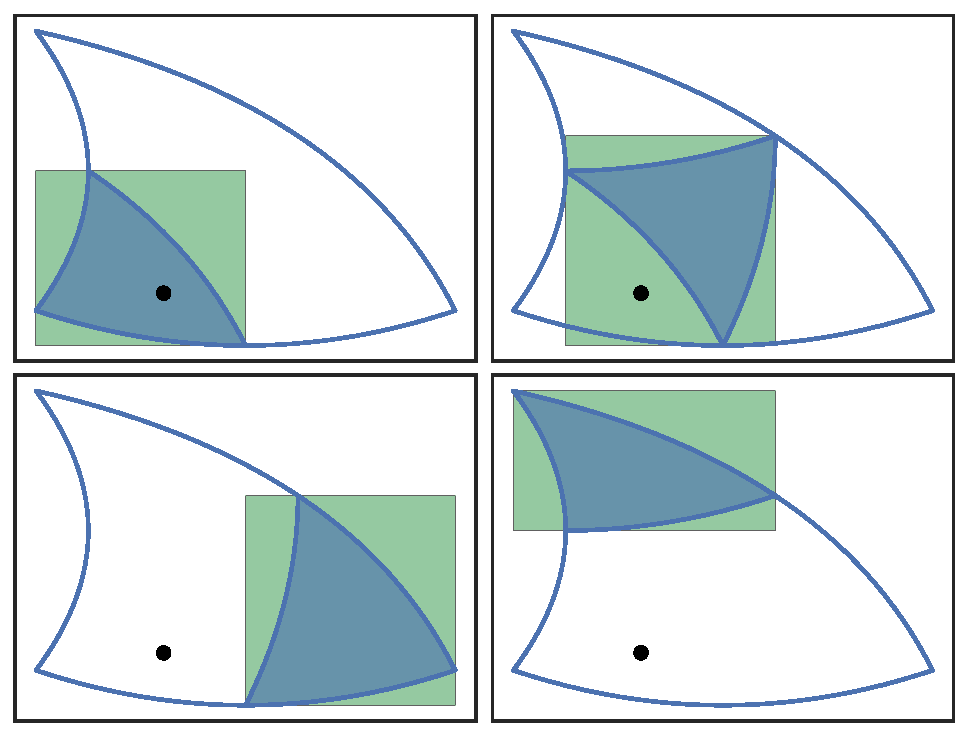
\includegraphics{../images/curved-mesh/locate_in_triangle.pdf}
  \centering
  \captionsetup{width=.75\linewidth}
  \caption{Checking for a point \(\bm{p}\) in each of four subregions
    when subdividing a B\'{e}zier triangle.}
  \label{fig:locate-in-triangle}
\end{figure}

For example, Figure~\ref{fig:locate-in-triangle} shows
how regions of \(\utri\) can be discarded recursively until the
suitable region for \((s, t)\) has a sufficiently small area. At
this point, we can apply Newton's method to the map \(F(s, t) =
b(s, t) - \bm{p}\). It's very helpful (for Newton's method) that
\(F: \reals^2 \longrightarrow \reals^2\) since the Jacobian will
always be invertible
when the B\'{e}zier triangle is valid. If \(\bm{p} \in \reals^3\)
then the system would be underdetermined. Similarly, if
\(\bm{p} \in \reals^2\) but \(b(s)\) is a B\'{e}zier curve then the
system would be overdetermined.
